\documentclass[tikz,border=5pt]{standalone}

\usetikzlibrary{automata, positioning, arrows.meta}

\begin{document}

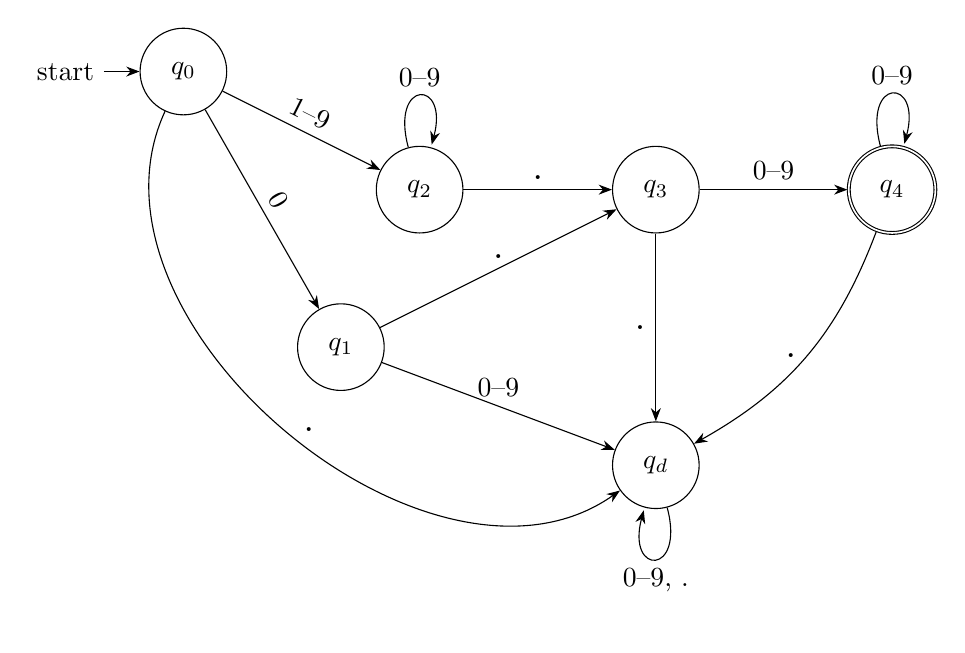
\begin{tikzpicture}[
    ->,
    >=Stealth,
    every state/.style={
        draw,
        circle,
        minimum size=1.1cm
    }
]

\node[state, initial] (q0) at (0,0) {$q_0$};
\node[state] (q1) at (2,-3.5) {$q_1$};
\node[state] (q2) at (3,-1.5) {$q_2$};
\node[state] (q3) at (6,-1.5) {$q_3$};
\node[state, accepting] (q4) at (9,-1.5) {$q_4$};
\node[state] (qd) at (6,-5) {$q_d$};

\path
(q0) edge node[above, sloped] {0} (q1)
(q0) edge node[above, sloped] {1--9} (q2)
(q0) edge[bend right=75] node[right=0.1cm, font=\LARGE] {.} (qd);

\path
(q1) edge node[above, font=\LARGE] {.} (q3)
(q1) edge node[above] {0--9} (qd);

\path
(q2) edge[loop above] node{0--9} ()
(q2) edge[above] node[font=\LARGE]{.} (q3);

\path
(q3) edge[above] node{0--9} (q4)
(q3) edge node[left, font=\LARGE]{.} (qd);

\path
(q4) edge[loop above] node{0--9} ()
(q4) edge[bend left=20] node[left, font=\LARGE] {.} (qd);

\path
(qd) edge[loop below] node{0--9, .} ();

\end{tikzpicture}

\end{document}